\documentclass[11pt]{article}
\usepackage{graphicx}
\usepackage{amsmath,amsthm,amsfonts}
\usepackage{epsfig,graphics}
\usepackage{hyperref}
\usepackage{verbatim}
\usepackage{mathrsfs}
\usepackage{fancyhdr}

\setlength{\textheight}{8.5in}
\setlength{\evensidemargin}{0.0in}
\setlength{\oddsidemargin}{0.0in}
\setlength{\topmargin}{-0.5in}
\setlength{\textwidth}{6.5in}

\newtheorem{theorem}{Theorem}
\newtheorem*{theorem*}{Theorem}
\newtheorem{claim}{Claim}
\newtheorem*{claim*}{Claim}
\newtheorem{lemma}{Lemma}
\newtheorem*{lemma*}{Lemma}
\newtheorem{exercise}{Exercise}
\newtheorem*{exercise*}{Exercise}
\newtheorem{corollary}{Corollary}
\theoremstyle{definition}
\newtheorem{definition}{Definition}
\newtheorem{fact}{Fact}
\newtheorem*{fact*}{Fact}


\pagestyle{fancy}
\fancyhf{}

%\newcommand{\lecture}[5]{\handout{#1}{#2}{#3}{#4}{#5}}


% Types of Variables
\newcommand{\bvar}[1]{\mathbf{#1}} % bold variable
\newcommand{\mvar}[1]{\bvar{#1}} % matrix variable
\newcommand{\vvar}[1]{\vec{#1}} % vector variable

% Domains
\newcommand{\R}{\mathbb{R}}
\newcommand{\Z}{\mathbb{Z}}
\newcommand{\redgevec}{\R^{E}}
\newcommand{\rvertvec}{\R^{V}}
\newcommand{\rPos}{\R^{+}}
\newcommand{\rNonNeg}{\R^{\geq 0}}

% Probability Operators
\newcommand{\E}{{\mathbb{E}}}
\newcommand{\V}{{\text{Var}}}
\newcommand{\prob}{{\mathbb{P}}}

% Symbol for definitions
\newcommand{\defeq}{\stackrel{\mathrm{\scriptscriptstyle def}}{=}}

% Optimization
\DeclareMathOperator*{\argmin}{arg\,min}
\DeclareMathOperator{\Cone}{Cone}
\DeclareMathOperator{\Cut}{CUT}

% Types of Graphs
\newcommand{\nlap}{\mathscr{L}_G}
\newcommand{\pseudo}[1]{{#1}^\dagger}
\newcommand{\lapPseudo}{\pseudo{\lap}}
\newcommand{\adj}{A}
\newcommand{\incMatrix}{\mvar{B}}
\newcommand{\diag}{\operatorname{diag}}
\newcommand{\rMatrix}{\mvar{R}} % resistance matrix
\newcommand{\iMatrix}{\mvar{I}} % identity matrix
\newcommand{\Vol}{\textrm{Vol}}


% Vectors
\newcommand{\1}{\vec{1}}
\renewcommand{\dot}[1]{\langle {#1} \rangle}

%other
\DeclareMathOperator{\sgn}{sgn}


\usepackage{wrapfig}
\graphicspath{{pictures/}}


\lhead{MA 881: Homework 1}
\rhead{Benjamin Draves}

\begin{document}

\section{Exercise 1: Testing Transcript Abundance}

Recall from class we developed an estimator for a transcript abundance vector $\vec{\rho}_t$ where $t\in T$ the transcript set. To simplify calculations, we partitioned the genome $\mathcal{G} = \bigcup_{i=1}^{|\mathcal{G}|}G_i$ and estimated the probability $\beta_g\equiv\prob(L_i = g)$ by $\hat{\beta}_g = \frac{X_g}{R}$ where $X_g$ is the number of fragments in region $G_g$ and $R$ is the total number of fragments produced by the aligning software. Next, we defined $L_i$ to be the true, but unobserved, region that the fragment $f_i$ belongs to. From here we constructed estimates for the transcript abundances written in fragments per kilobase of transcript per million fragments mapped (FPKM). This estimate is given by 
\begin{equation}
\hat{\rho_t}\propto \frac{10^9X_g\hat{\gamma_t}}{\tilde{L}(t)R}
\end{equation}
where $\tilde{L}(t)$ is the adjusted length of transcript $t$ and $\gamma_t = \prob(f_i = r_i|L_i = g, T_i = t)$ is estimated by constrained maximum likelihood of $\mathcal{L}(\vec{\rho}|T)$. In class, we constructed a test to determine if there was an observable difference between two group means. That is we constructed a test statistic to infer if there was a difference between transcript abundances for two different treatment groups across a fixed transcript. We wish to generalize this concept to testing multiple treatments. For concreteness consider the following data matrix.
\begin{figure}[h!]
	\centering
	\begin{tabular}{|c|c|c|c|c|c|}
	\hline
		Transcript & Control & Treatment 1 & Treatment 2 & \ldots & Treatment $n$\\
		\hline
		$t_1$ & $c_{1}$ & $m^{(1)}_{1}$ & $m^{(2)}_{1}$ & \ldots & $m^{(n)}_{1}$\\
		$t_2$ & $c_{2}$ & $m^{(1)}_{2}$ & $m^{(2)}_{2}$ & \ldots & $m^{(n)}_{2}$\\
		\vdots &\vdots &\vdots &\vdots &\vdots &\vdots\\
		\hline  
	\end{tabular}
	\caption{Observed transcription matrix}
\end{figure}
Here, assuming that each treatment only has a single individual, we wish to test the abundances corresponding to each entry of the \textit{rows} of this matrix. The relevent hypotheses are stated below. 
\begin{align}
H_0&: \rho_t^{(1)} = \rho_t^{(2)} = \dots = \rho_t^{(n)}\\
H_1&: \text{There exists at least one $i$ such that $\rho_t^{(i)} \neq \rho_t^{(j)}$}
\end{align} 

Now to develop a test statistic, we first note that under the null hypothesis $\E(\overline{\rho_t}) = \E(\rho_t^{(i)})$ for all $1\leq i \leq n$. Hence we can construct statistics that follow the Wald statistic construction as follows 
\begin{equation}
\hat{\theta}_{t}^{(i)} = \frac{\hat{\rho}_t^{(i)} - \overline{\rho_t}}{\widehat{\V(\rho_t^{(i)})}}\overset{\cdot}{\sim}N(0,1)
\end{equation}
Taking this approximation, we see that the sum, along with Cochran's theorem gives the following 
\begin{equation}
	T\equiv \sum_{i=1}^n\left[\hat{\theta}_t^{(i)}\right]^2 = \sum_{i = 1}^n \left(\frac{\hat{\rho}_t^{(i)} - \overline{\rho_t}}{\widehat{\V(\rho_t^{(i)})}}\right)^2\overset{\cdot}{\sim} \chi^2_{n-1}
\end{equation}
From here, we can carry out statistical tests based on the test statistic $T$. That is, for some criticial value based on $\alpha$, $\chi^2_{n-1, 1-\alpha}$ we build the decision rule as follows. 
\begin{equation}
	D(\hat{\vec{\rho_t}},\alpha) = \begin{cases}
	\text{Reject $H_0$} & T(\hat{\vec{\rho_t}})\in (\chi^2_{n-1, 1 -\alpha}, \infty)\\
	\text{Fail to reject $H_0$} & T(\hat{\vec{\rho_t}})\in (0,\chi^2_{n-1, 1 -\alpha})\\
	\end{cases}
\end{equation}
This procedure can be extended to include multiple samples within each treatment group. If we have multiple samples within each group, we could instead calculate the ratio of the between treatment group variability over the within treatment group variability. This test would follow a typicall $F$ type test and would test the hypothesis if the transcript abundance was different between treatment groups and not individuals as we have presented here.

\section{Exercise 2: Combining Gene-Read Estimators}

\begin{wrapfigure}{R}{0.5\textwidth}
	\centering
	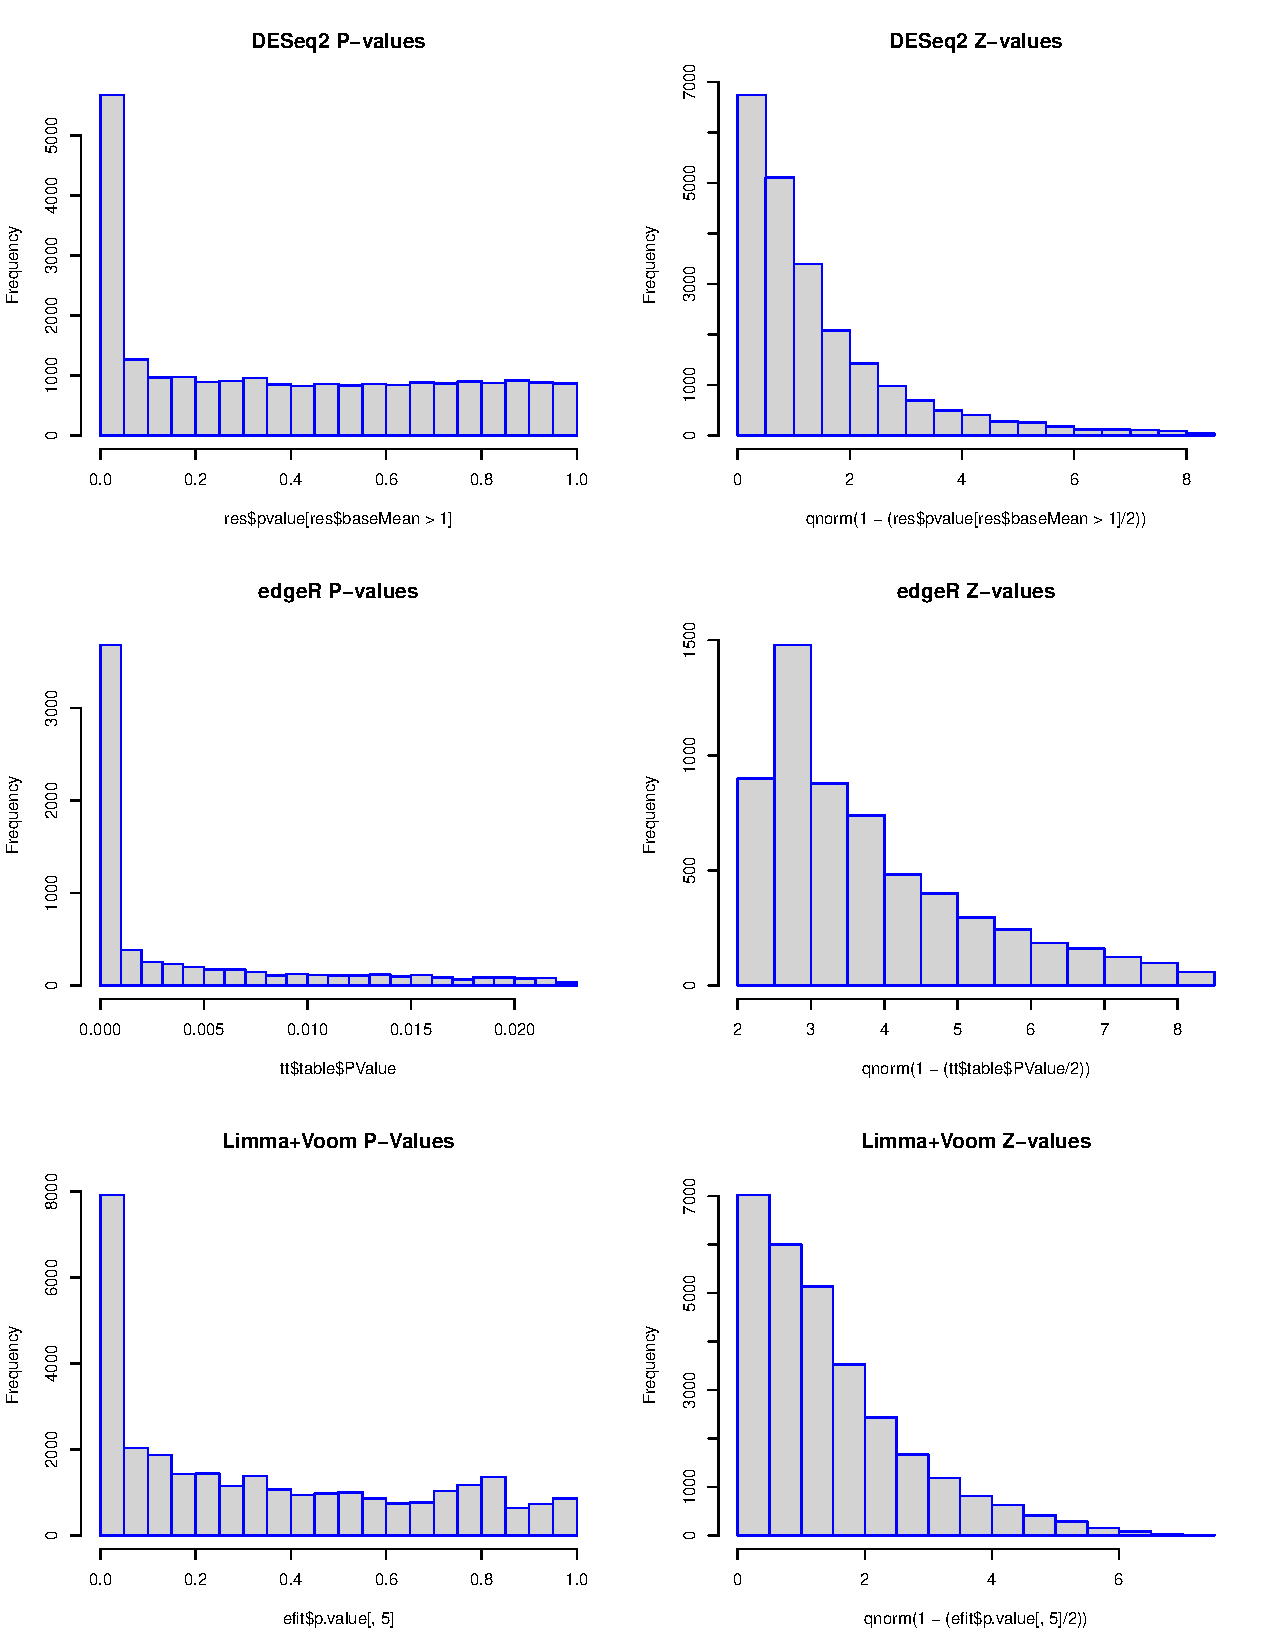
\includegraphics[scale = 0.4]{code/p_value_hist.pdf}
	\caption{Histograms $p-values$ and associated (positive) z-scores for each of the three methods considered.}
\end{wrapfigure}
The airway dataset is an open source dataset provided by the Bioconductor package. The dataset contains a gene-read matrix for an RNA-seq experiment on four human airway muscle cell lines that have been treated. n the left column of Figure 2 are the resulting $p$-value histograms from testing the differences betweens genes for the treated airway cell lines and the treated cell lines. In the right column are the associated positive $z$ statistics for each of the three methods considered; DESeq2, edgeR, and Limma+Voom. 

It appears that edgeR overfits and is quite liberal, rejecting null hypothesis. That is, several tests appear to be rejecting, more than likely falsely. DESeq2 appears to partition the data into active versus inactive genes. We have several p-values all clustered at zero then a uniform p-value distribution over the remainder of the interval $[0,1]$. Limma+Voom appears to exhibit behavior as the mix between the two. That is, the method is detecting signal in several genes as evident by the number of small p-values. Moreover, there appears to be more variability in the remainder of the p-values. This could be due to the way that Limma+Voom disregards the count nature of the data and instead treats the data linearly. Hence we could be seeing this more continuous nature in the p-values as a result of this modeling choice. 

The three methods provide three separate hypothesis tests for each gene in the genome. Our goal is to consolidate these tests into a single informed decision about whether the gene in question plays a role in the difference between the treatment versus control groups. One naive approach to this problem is \textit{committee voting} where we simply choose to reject if the majority of tests reject the hypothesis. A more probabilistically informed approach can be done by summing the $p$-values. Under the null hypothesis $p_t^{(i)}\sim\text{Unif}(0,1)$. Hence, if we take the associated $p$-values as independent we have the following result 
\begin{equation}
p_t^{(edgeR)} + p_t^{(DESeq2)} + p_t^{(LV)} \sim \begin{cases}
\frac{x^2}{2} & 0<x<1\\
-x^2+3x-\frac{3}{2} & 1<x<2\\
-\frac{(w-3)^2}{2} & 2<x<3\\
\end{cases}  
\end{equation}
Now, clearly these p-values are not independent as they are all determined by the same gene activity. However, if we naively assume that these values are independent, we can use the distribution in $(7)$ to preform testing on these aggregated $p$-values. By doing so, we require that the gene in question needs to demonstrate significance activity across all three models to be discovered by the consolidation of these three models. Perhaps weighting these $p$-values based on the model fit statistics of each edgeR, DESeq2, and Limma+Voom, we could build a more robust consolidation technique that also incorporates flaws in the modeling assumptions made by these three methods.  




\end{document}







